\documentclass{beamer}

\mode<presentation> {

\usetheme{Madrid}

\setbeamertemplate{footline} % To remove the footer line in all slides uncomment this line

\setbeamertemplate{navigation symbols}{} % To remove the navigation symbols from the bottom of all slides uncomment this line
}

\usepackage{minted} % syntax highlighting for haskell expressions
\usepackage{graphicx} % Allows including images
\usepackage{booktabs} % Allows the use of \toprule, \midrule and \bottomrule in tables
\usepackage[utf8]{inputenc}

%----------------------------------------------------------------------------------------
%	TITLE PAGE
%----------------------------------------------------------------------------------------

\title[Conditional Conjectures in QuickSpec]{Conditional Conjectures in QuickSpec} % The short title appears at the bottom of every slide, the full title is only on the title page

\author{Maximilian Algehed} % Your name
\institute[CTH] % Your institution as it will appear on the bottom of every slide, may be shorthand to save space
{
Chalmers University of Technology \\ % Your institution for the title page
\medskip
\textit{m.algehed@gmail.com} % Your email address
}
\date{\today} % Date, can be changed to a custom date

\begin{document}

\begin{frame}
    \titlepage % Print the title page as the first slide
\end{frame}

\begin{frame}
    \frametitle{What is QuickSpec?}
    \begin{columns}
        \column{0.15\textwidth}
        \begin{block}{}
            Functions\\
            Datatypes\\
            Constants\\
        \end{block}

        \column{0.1\textwidth}
        \\
        \centerline{\Large{$\implies$}}

        \column{0.15\textwidth}
        \begin{block}{}
            QuickSpec
        \end{block}
        
        \column{0.1\textwidth}
        \\
        \centerline{\Large{$\implies$}}

        \column{0.15\textwidth}
        \begin{block}{}
            Equations
        \end{block}
    \end{columns}
\end{frame}

\begin{frame}
    \frametitle{Demo!}
        \Huge{\centerline{Demo!}}
\end{frame}

\begin{frame}
    \frametitle{How does it do this?}
        \begin{itemize}
            \item Test terms against each other\\\texttt{xs ++ (ys ++ zs) = (xs ++ ys) ++ zs}
            \item QuickSpec tests the most general terms first\\
                \texttt{xs ++ (ys ++ zs) = (xs ++ ys) ++ zs}\\implies\\\texttt{xs ++ (xs ++ xs) = (xs ++ xs) ++ xs}
            \item Uses fast equational reasoning to determine\\if it needs to test a term at all
        \end{itemize}
\end{frame}

\begin{frame}
    \frametitle{What's this?}
        \Large{\centerline{\texttt{zip xs (xs ++ ys) = zip xs xs}}}
\end{frame}

\begin{frame}
    \frametitle{What we'd like}
    \Large{\centerline{\texttt{length xs = length ys =>}}
    \centerline{\texttt{zip xs (ys ++ js) = zip xs ys}}}
\end{frame}

\begin{frame}
    \frametitle{Demo!}
        \Huge{\centerline{Demo!}}
\end{frame}

\begin{frame}[fragile]
    \frametitle{How does it work?}
    \begin{minted}{haskell}
data Peqlen = Peqlen {xs :: [Int],
                      ys :: [Int]}

instance Arbitrary Peqlen where
    arbitrary = do
                    l  <- arbitrary 
                    xs <- sequence $
                        replicate l arbitrary
                    ys <- sequence $
                        replicate l arbitrary
                    return (Peqlen xs ys)
        \end{minted}

\end{frame}

\begin{frame}
    \frametitle{How does it work?}
    \Large{\centerline{\texttt{length xs = length ys =>}}}
    \Large{\centerline{\texttt{zip xs (ys ++ is) = zip xs ys}}}
        \centerline{}
        \centerline{becomes}
        \centerline{}
        \Large{\centerline{\texttt{zip (xs p) (ys p ++ is) = zip (xs p) (ys p)}}}
        \pause
        \centerline{}
        \centerline{\texttt{zip (ys p) (xs p ++ is) = zip (ys p) (xs p)}}
        \centerline{}
        \centerline{(We have a fix for this in the pipeline!)}
\end{frame}

\begin{frame}
    \frametitle{So what about redundancy?}
        \Large{\centerline{\texttt{f z = g (x p)}}}
        \centerline{}
        \centerline{more general than}
        \centerline{}
        \Large{\centerline{\texttt{f (y q) = g (x p)}}}
\end{frame}

\begin{frame}
    \frametitle{Theory exploration intermission}
    \begin{columns}
        \column{0.15\textwidth}
        \begin{block}{Isabelle}
            \small{Need lemmas to prove target}
        \end{block}

        \column{0.1\textwidth}
        \\
        \centerline{Definitions}
        \centerline{\Large{$\implies$}}
        \centerline{\Large{$\impliedby$}}
        \centerline{Lemmas}

        \column{0.15\textwidth}
        \begin{block}{Hipster}
            \small{Prove conjectures inductively}
        \end{block}
        
        \column{0.1\textwidth}
        \\
        \centerline{Definitions}
        \centerline{\Large{$\implies$}}
        \centerline{\Large{$\impliedby$}}
        \centerline{Conjectures}

        \column{0.2\textwidth}
        \begin{block}{QuickSpec}
            \small{Conjecture conjectures
            \\(we are here)}
        \end{block}

    \end{columns}
\end{frame}

\begin{frame}[fragile]
    \frametitle{Generalizing, the naive way}
    \begin{minted}{haskell}
arbitrary = do
    (xs, ys) <- arbitrary `suchThat`
                (\(xs, ys) -> length xs == length ys)
    return $ Peqlen xs ys
        \end{minted}   
\end{frame}

\begin{frame}
    \frametitle{Demo!}
        \Huge{\centerline{Demo time!}}
\end{frame}

\begin{frame}[fragile]
    \frametitle{APL}
        \Huge{\centerline{APL}}
        \pause
        \small{\centerline{you know, that language...}}
        \centerline{}
        \centerline{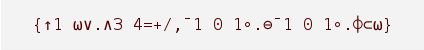
\includegraphics[scale=0.5]{game_of_life.png}}
\end{frame}

\begin{frame}
    \frametitle{APL}
    \begin{columns}
        \column{.5\textwidth}
            Problem: I don't understand APL\\

        \pause

        \column{.5\textwidth}
            Solution: I understand haskell...\\
            Deep embedding? NO!\\
            Shallow embedding
    \end{columns}
\end{frame}

\begin{frame}
    \frametitle{Something more interesting}
        In APL, the $\rho$ operator gets the shape of a value.\\
        \begin{align*}
        \rho\;\begin{pmatrix} 0 & 2 & 1 \end{pmatrix}\; &= \begin{pmatrix}3\end{pmatrix}\\\\
            \rho \begin{pmatrix} 2 & 1 \\ 3 & 4 \end{pmatrix} &= \begin{pmatrix} 2 & 2\end{pmatrix}\\\\
            \rho \begin{pmatrix} 2 & 1 \\ 1 \end{pmatrix} &= crash...
        \end{align*}
\end{frame}

\begin{frame}
    \frametitle{Something more interesting}
        The $\times$ operator does element wise multiplication.\\
        \begin{align*}
            \begin{pmatrix} 1 & 2\\3 & 4\end{pmatrix} \times \begin{pmatrix} 2 & 3\\6 & 2\end{pmatrix} &=
            \begin{pmatrix} 2 & 6\\18 & 8\end{pmatrix}\\\\
            \begin{pmatrix} 1 & 4 & 3 \end{pmatrix} \times \begin{pmatrix}1 & 0 & 0 & 1 \end{pmatrix} &= crash...
        \end{align*}
\end{frame}

\begin{frame}
    \frametitle{Something more interesting}
        \centerline{What we expect}
        \begin{equation*}
            \rho (x \times y) = \rho x = \rho y
        \end{equation*}
        \centerline{}
        \centerline{for all well behaved x and y...}
\end{frame}

\begin{frame}
    \frametitle{Being well behaved}
        \begin{columns}
            \column{.5\textwidth}
                \begin{itemize}
                    \item $\rho x$ does not crash
                    \item $\rho y$ does not crash
                    \item $\rho x = \rho y$
                \end{itemize}
            \column{.5\textwidth}
                \pause
                \centerline{\texttt{suchThat} won't cut it}
                \centerline{}
                \centerline{Let's go back to doing it by hand...}
        \end{columns}
\end{frame}

\begin{frame}
    \frametitle{Demo!}
        \Huge{\centerline{Demo!}}
\end{frame}

\begin{frame}
    \frametitle{We need better generators}
        Area of research
        \begin{itemize}
            \item enumeration - \texttt{FEAT}
            \item laziness - \texttt{Generating constrained random data}
            \item laziness \& enumeration - \texttt{Lazy SmallCheck}
            \item constraint solving - \texttt{Making our own luck}
        \end{itemize}
        Writing predicate $\iff$ Writing generator\\
        \centerline{}
        Order of generation
        \begin{itemize}
            \item order by importance
            \item weighted random order
        \end{itemize}
\end{frame}

\begin{frame}
    \frametitle{Injectivity}
        \begin{block}{Injectivity}
            \centerline{"$f$ is injective"}
            \centerline{$\iff$}
            \centerline{$f\;x=f\;y\implies x = y$}
            \centerline{$\iff$}
            \centerline{$x \neq y \implies f\;x\neq f\;y$}
        \end{block}
\end{frame}

\begin{frame}[fragile]
    \frametitle{Algebraic expressions}
    \begin{minted}{haskell}
    data Expression = Expression :+: Expression
                    ...
                    | X

    showexp :: Expression -> String
    ...
    showexp (a :+: b) = "(" ++
                         (showexp a) ++ " + " ++ (showexp b)
                         ++ ")"
    \end{minted}
\end{frame}

\begin{frame}
    \frametitle{Demo!}
        \Huge{\centerline{Demo!}}
\end{frame}

\begin{frame}[fragile]
    \frametitle{April's fools!}
    \begin{minted}{haskell}
    data Expression = Expression :+: Expression
                    ...
                    | X

    showexp :: Expression -> String
    ...
    showexp (a :+: b) = (showexp a) ++ " + " ++ (showexp b)
    \end{minted}
\end{frame}

\begin{frame}
    \frametitle{Demo!}
        \Huge{\centerline{Demo!}}
\end{frame}

\begin{frame}
    \frametitle{Oh dear, what a mess!}
    \begin{itemize}
        \item Hand written generator
        \item \texttt{mutate}...
        \item Need to be specific
    \end{itemize}
\end{frame}

\begin{frame}
    \frametitle{The other way}
    \centerline{$x \neq y \implies f\;x\neq f\;y$} 
\end{frame}

\begin{frame}
    \frametitle{Demo!}
        \Huge{\centerline{Demo!}}
\end{frame}

\begin{frame}
    \frametitle{YAY!}
    \centerline{It found the bug, right?}
    \pause
    \centerline{}
    \centerline{\texttt{xs /= show e = True} $\implies$ \texttt{show (e p) /= show (f p) = True}}
    \centerline{}
    \centerline{We don't know if it found the bug, because it never tested for the bug}
\end{frame}

\begin{frame}
    \frametitle{Summary}
    \begin{itemize}
        \item QuickSpec only supports equations
        \item Types with invariants introduce conditionals
        \item We need fast generation of constrained random data
    \end{itemize}
\end{frame}

\begin{frame}
    \Huge{\centerline{Questions?}}
\end{frame}

\end{document} 
